\documentclass[a5paper,ngerman]{article}
\usepackage[T1]{fontenc}
\usepackage[utf8]{inputenc}
\usepackage[margin=0.5in,includefoot]{geometry}
\usepackage{microtype}
\usepackage{babel}
\usepackage{siunitx}
\usepackage[dark]{solarized}
\usepackage{sectsty}
\usepackage{ccfonts}
\usepackage{euler}
\usepackage{fancyhdr}
\usepackage{fancyvrb}
\usepackage{graphicx}
\usepackage{multicol}
\usepackage{mdframed}
\usepackage{lisp}
\pagestyle{fancy}
\fancypagestyle{plain}{
\fancyhf{}
\fancyfoot[C]{{\color{deemph}\small$\thepage$}}
\renewcommand{\headrulewidth}{0pt}
\renewcommand{\footrulewidth}{0pt}}
\title{\color{emph}Am Anfang war der Arbeitsspeicher}
\author{Timm Knape}
\date{\today}
\columnseprule.2pt
\renewcommand{\columnseprulecolor}{\color{deemph}}
\begin{document}
\pagecolor{background}
\color{normal}
\allsectionsfont{\color{emph}\mdseries}
\pagestyle{plain}
\maketitle
\thispagestyle{fancy}
\surroundwithmdframed[backgroundcolor=codebackground,fontcolor=normal,hidealllines=true]{Verbatim}

Bevor wir die zentrale Arbeitseinheit (central processing unit = CPU)
in Betrieb nehmen können,
müssen wir ihr einer Umgebung schaffen, in der sie sich wohlfühlt.

Dazu gehört erst eine Form von Speicher.
Aus dem Speicher liest die CPU Befehle und Daten.
Auch Ergebnisse kann sie dort ablegen.

Es gibt viele Arten von Speicher.
Mancher behält seinen Inhalt, wenn er nicht mit Strom versorgt wird.
Andere können nur einmal beschrieben werden.
Oder müssen aufwändig mit UV-Licht gelöscht werden.
Gebräuchliche Bausteine müssen mehrmals pro Sekunde neu beschrieben
werden, da sie sonst ihren Inhalt vergessen.

Wir fangen mit einem einfachen statischen RAM-Baustein an.
RAM steht für random access memory.
Das ist Speicher, der gelesen und beschrieben werden kann.

Wichtig ist, dass er eine Versorgungsspannung von 5 Volt hat.
Und dass er mindestens acht Zustände zu jeder Adresse hinterlegen kann.

Ich verwende einen NEC D431000ACZ-70LL, den ich für ein paar Euro bei
Ebay erstanden habe.

Dieser hat die folgende Pin-Belegung:

\centerline{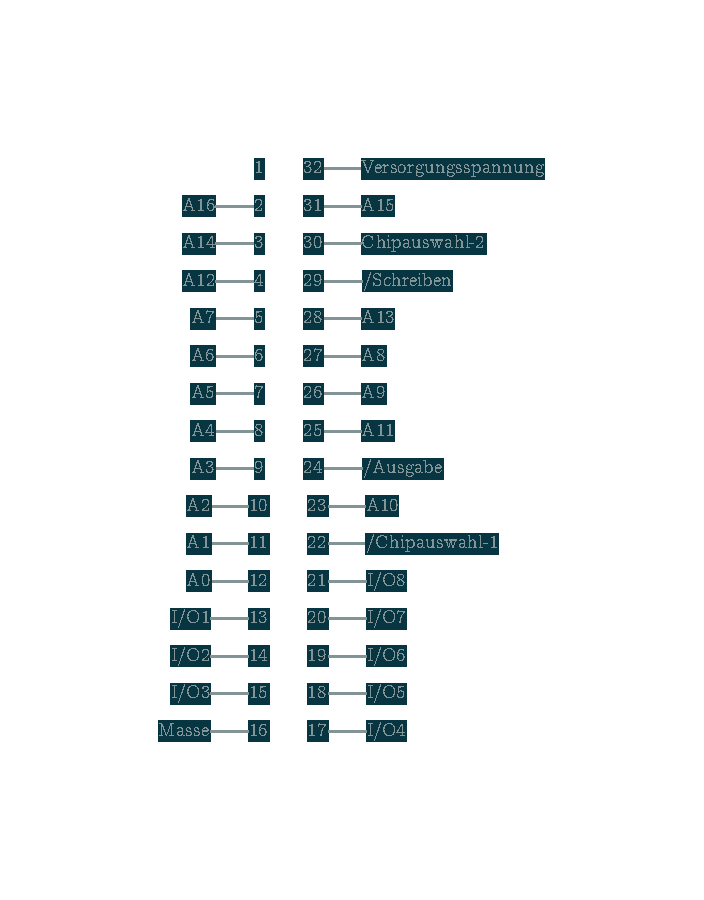
\includegraphics[trim={1in .9in 1in .9in},clip]{imgs/dot-1-dark.pdf}}
\end{document}
